\documentclass{article}
\usepackage[utf8]{inputenc}
\usepackage{amsmath}
\usepackage{amsthm}
\usepackage{amssymb}
\usepackage{graphicx}
\usepackage{subcaption}
\usepackage{float}
\usepackage{tikz}
\usepackage{caption}

\captionsetup{width=0.75\linewidth}

\newcommand{\w}{0.5}
\newcommand{\ww}{0.25}

\newcommand{\drawgrid}[2]{\draw[step=\w cm,black,thin] (0,0) grid (#1*\w,#2*\w);}
\newcommand{\drawgraygrid}[2]{\fill[fill=gray!40!white] (0,0) rectangle (#1*\w,#2*\w); \draw[step=\w cm,black,thin] (0,0) grid (#1*\w,#2*\w);}

\newcommand{\labelcol}[2]{\draw (#1*\w cm - \ww cm, 0 cm) node[anchor=north] {#2};}
\newcommand{\labelrow}[2]{\draw (0 cm, #1*\w cm - \ww cm) node[anchor=east] {#2};}

\newcommand{\placerook}[2]{\draw (#1*\w cm - \ww cm, #2*\w cm - \ww cm) node {$R$};}
\newcommand{\places}[2]{\draw (#1*\w cm - \ww cm, #2*\w cm - \ww cm) node {$s$};}
\newcommand{\placelabel}[3]{\draw (#1*\w cm - \ww cm, #2*\w cm - \ww cm) node {#3};}

\newcommand{\shadesquare}[2]{\filldraw[fill=gray!40!white, draw=black] (#1*\w - \w,#2*\w - \w) rectangle (#1*\w,#2*\w);}
\newcommand{\unshadesquare}[2]{\filldraw[fill=white, draw=black] (#1*\w - \w,#2*\w - \w) rectangle (#1*\w,#2*\w);}

\newtheorem{definition}{Definition}
\newtheorem{lemma}{Lemma}
\newtheorem{theorem}{Theorem}

\title{MATH333 Final Project: Rook Polynomials}
\author{Oliver Calder, Risa Fines}
\date{March 2020}

\begin{document}

\maketitle

\section{Introduction to Rook Numbers} \label{intro}
A rook is a type of chess piece that can move only along the column or row it is in, and so can only capture another chess piece which is in the same column or row as it is. A single space on any board may not be occupied by more than one rook. Therefore, in order to place some number of rooks on an otherwise empty board (that is, a board with no chess pieces present) such that no rook will be able to capture any other rook, each row or column can have no more than one rook present.

\begin{definition} A \textbf{board} is a set of squares arranged in rows and columns (as on a chessboard) such that ``rooks" may only be placed on squares within this set. A \textbf{subboard} $B_1$ of a board $B$ is a board composed of a subset of the squares in $B$.
\end{definition}

In the diagrams which follow in this paper, squares which are part of the given board are darkened, while there may remain white squares to indicate alignment of rows or columns. Note that boards need not resemble $n \times n$ chessboards, but the squares in the board may take any form so long as they remain in definite rows and columns.

\begin{definition}
    A \textbf{rook number} is the number of ways to place $k$ rooks on a given board $B$ such that each row and column of the board each have at most one rook. The rook number for a given $k$ and $B$ is denoted $r_k(B)$. The rooks on such a board can be said to be ``mutually non-capturing".
    
    By convention, because there is one way to place zero rooks on any given board, $r_0(B)= 1$ for all $B$.
\end{definition}


\section{Placing Rooks on ``Simple" Boards} \label{simple}

\begin{figure}
    \centering
    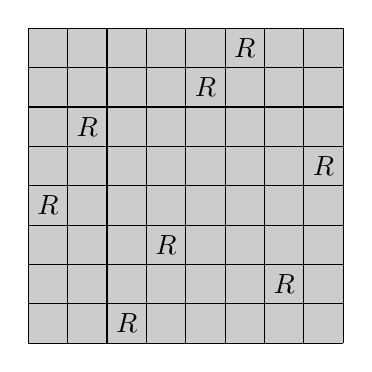
\begin{tikzpicture}
        \drawgraygrid{8}{8};
        \placerook{3}{1};
        \placerook{7}{2};
        \placerook{4}{3};
        \placerook{1}{4};
        \placerook{8}{5};
        \placerook{2}{6};
        \placerook{5}{7};
        \placerook{6}{8};
    \end{tikzpicture}
    \caption{An $8 \times 8$ board with $8$ non-capturing rooks.}
    \label{chessboard}
\end{figure}

Given a board with n rows and n columns, where a rook may be placed onto any square, how many ways are there to place $k$ (with $0 \leq k \leq n)$ mutually non-capturing rooks on this board? An example of this can be seen in Figure \ref{chessboard}. We may break this question into several components. First, we must choose onto which of the $n$ rows we will place our $k$ rooks. Since we cannot choose the same row more than once, and the order in which we choose the rows does not matter, the number of ways to choose $k$ rows from $n$ total rows will be given by $\binom{n}{k}$. We can use the same process to determine onto which of the columns our $k$ rooks will be placed, so this is also given by $\binom{n}{k}$. Thus, the total number of ways to choose the $k$ rows and $k$ columns is given by $\binom{n}{k}\binom{n}{k}$.

Now, we have a set of possible squares onto which our rooks may be placed. Pick some arbitrary row out of the $k$ rows you've selected. Then there are $k$ ways to place a rook in this row since there are $k$ available columns in this row and no other rooks have yet been placed. Proceed to another row. Since a rook has already been placed in one of the columns, another rook cannot be placed in that same column, so there are $k-1$ ways to place a rook in this row. We can generalize: for the $i^{th}$ rook you are placing, there will be $k-i$ ways to place this rook on the board because $k-i$ rows and columns will be occupied by the previous rooks you have placed. Thus, the number of ways to place $k$ rooks given $k$ rows and $k$ columns is $k \times (k-1) \times (k-2) \times ... \times (k - i) \times ... \times 1 = k!$.

Therefore, the total number of ways to place $k$ rooks on an $n \times n$ board is given by \begin{equation} \label{unrestricted}
    \binom{n}{k} \binom{n}{k} k!
\end{equation}

This problem becomes more complex when you limit the positions in which the rooks may be placed on the board. We may call any square where a rook may not be placed ``unavailable". Take, for example, a $4\times4$ grid where the top left corner is unavailable, as in Figure \ref{topleftunavailable}.
\begin{figure}[!h]
    \centering
    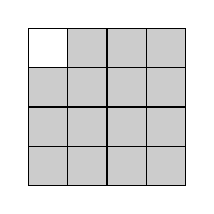
\begin{tikzpicture}
        \drawgraygrid{4}{4};
        \unshadesquare{1}{4};
    \end{tikzpicture}
    \caption{A chessboard where the top left square is ``unavailable".}
    \label{topleftunavailable}
\end{figure}

Let us try to place four rooks on this board in order to build an intuition for a way to approach calculating the rook numbers of small boards which have some unavailable squares.

In the example given by \ref{topleftunavailable}, we can see that in the top row, we have three choices for the placement of a rook. For the next row, we have three choices, since all columns are available except the one in which a rook was placed in the first row. Similarly, we have two choices for the third row, and one choice for the final row. Thus, the total number of ways to place four rooks on the board is given by $3\times3\times2\times1=18$.

However, what if there are unavailable tiles elsewhere in the board such that we cannot so easily count the number of ways to place non-capturing rooks on the board, as we did for the board in Figure \ref{topleftunavailable}? Such a board is shown in Figure \ref{internal}.

\begin{figure}[h!]
    \centering
    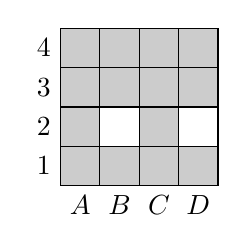
\begin{tikzpicture}
        \drawgraygrid{4}{4};
        \foreach \i in {1, 2, 3, 4} \labelrow{\i}{\i};
        \labelcol{1}{$A$};
        \labelcol{2}{$B$};
        \labelcol{3}{$C$};
        \labelcol{4}{$D$};
        \unshadesquare{2}{2};
        \unshadesquare{4}{2};
    \end{tikzpicture}
    \caption{A chessboard with internal ``unavailable" squares.}
    \label{internal}
\end{figure}

In this case, it may be beneficial to our intuition if we rearrange some of the rows and columns of the board such that unavailable squares are ``clustered" together. Note that there is no inherent interaction between rows and columns, nor between distinct rows or distinct columns. In other words, the rows and columns are arbitrarily ordered on the board. Thus, we may arbitrarily rearrange rows and columns without affecting the rook number of the board. Figure \ref{rearranged} shows a rearrangement of the rows and columns of the board in Figure \ref{internal} so that the unavailable squares are clustered.

\begin{figure}[!h]
    \centering
    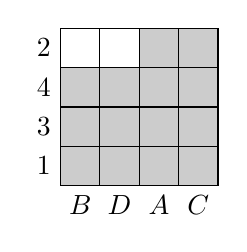
\begin{tikzpicture}
        \drawgraygrid{4}{4};
        \labelrow{1}{1};
        \labelrow{2}{3};
        \labelrow{3}{4};
        \labelrow{4}{2};
        \labelcol{1}{$B$};
        \labelcol{2}{$D$};
        \labelcol{3}{$A$};
        \labelcol{4}{$C$};
        \unshadesquare{1}{4};
        \unshadesquare{2}{4};
    \end{tikzpicture}
    \caption{A rearranged chessboard with ``unavailable" squares clustered.}
    \label{rearranged}
\end{figure}

Now, we may take the same approach to counting the number of ways to place four rooks as we took for figure \ref{topleftunavailable}.

\textsc{Note:} This is not a rigorous approach to solving problems of this variety. However, this provides an intuition about how to simplify problems such that the more rigorous tools we are about to develop can be applied more easily.

\section{Rook Polynomials}

Up to this point, we have considered how to count the number of ways to place a fixed $k$ number of rooks on a given board. However, we can also consider the number of ways to place $k$ non-capturing rooks for all $k \geq 0$. 

\begin{definition}
    A \textbf{rook polynomial} of a given board $B$ is a polynomial where the coefficient of the $x^k$ term is the number of ways to place $k$ non-capturing rooks on the board $B$. The rook polynomial, denoted $R(x, B)$, is thus given by
    \begin{equation}\begin{split} \label{rookpoly}
       R(x,B) &= r_0(B) + r_1(B)x + r_2(B)x^2 + ... \\
        &= \sum_{k=0}^{\infty} r_k(B) x^k
    \end{split}\end{equation}
\end{definition}
\textsc{Note:} A rook polynomial can be considered a ``generating polynomial" for the rook numbers. As we will see in Theorem 1, this means that rook polynomials behave much like generating functions. We can apply our knowledge of the behavior of products of generating functions to rook polynomials.

\begin{figure}[!h]
    \centering
    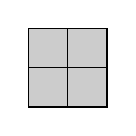
\begin{tikzpicture}
        \shadesquare{1}{1}
        \shadesquare{1}{2}
        \shadesquare{2}{2}
        \shadesquare{2}{1}
    \end{tikzpicture}
    \caption{An example board for which we can calculate the rook polynomial.}
    \label{2by2}
\end{figure}

Consider the $2\times2$ board $B$ in Figure \ref{2by2}. There will always be one way to place zero rooks on any board, so $r_0(B) = 1$. Since there are four tiles on our $2 \times 2$ board, there are four ways to place a single rook on $B$, so $r_1(B) = 4$. There are two ways to place two non-capturing rooks on $B$, so $r_2(B) = 2$. There is no possible way to put more than two mutually non-capturing rooks on a board with only 2 columns and 2 rows, so $r_k(B) = 0$ for $k>2$.

Thus, we can construct the rook polynomial for $B$ as follows:
\begin{align*}
R(x,B) &= r_0(B) + r_1(B)x + r_2(B)x^2 \\
& = 1 + 4x + 2x^2
\end{align*}

\pagebreak
\section{Decomposition into Disjoint Subboards} \label{decomposable}
It may be the case that we have a large board with many available squares scattered throughout the board. Rather than consider all the positions of the board as a whole, it may be of benefit to be able to split the board into subboards for which we are more easily able to calculate the rook numbers and rook polynomials.

\begin{definition}
    We define subboards $B_1$ and $B_2$ to be \textbf{disjoint subboards} if and only if there does not exist any square in $B_1$ that shares a row or column with any square in $B_2$. We refer to a board as \textbf{decomposable} if and only if it has two or more disjoint subboards.
\end{definition}

\begin{lemma}
    If $B$ is a board of darkened squares that decomposes into two disjoint subboards $B_1$ and $B_2$, then
    \begin{equation}\begin{split} \label{lem1}
        r_k(B) &= r_k(B_1)r_0(B_2) + r_{k-1}(B_1)r_1(B_2) + ... + r_0(B_1)r_k(B_2) \\
        &= \sum_{i=0}^{k}r_{k-i}(B_1)r_i(B_2)
    \end{split}\end{equation}
\end{lemma}

\begin{proof}
   We can show Lemma 1 combinatorially. Consider the ways to place $k$ rooks on B. All rooks will either be placed on $B_1$ or $B_2$. If there are $i$ rooks (such that $0 \leq i \leq k)$ placed on subboard $B_1$, then there will be $k-i$ rooks placed on subboard $B_2$. Because each subboard has unique rows and columns, the arrangement of rooks within $B_1$ is independent of the arrangement of rooks within $B_2$. Therefore, there are $r_i(B_1) r_{k-i}(B_2)$ ways to place $i$ rooks in $B_1$ and $k-i$ rooks in $B_2$. 
    
    To find the total number of ways to distribute $k$ rooks across a board $B$, we take the sum of the products of the rook numbers $r_i(B_1)$ and $r_{k-i}(B_2)$ for all possible values of $i$. Hence, 
    $$r_k(B) = \sum_{i=0}^{k}r_{i}(B_1)r_{k-i}(B_2)$$
\end{proof}

\begin{theorem}
    If $B$ is a board that decomposes into the two disjoint subboards $B_1$ and $B_2$, then
    \begin{equation} \label{thm1}
        R(x,B) = R(x,B_1)R(x,B_2)
    \end{equation}
\end{theorem}

\begin{proof}
    We have from the definition of a rook polynomial that $R(x,B) = \sum_{k=0}^{\infty} r_k(B) x^k$. We have from Lemma 1 that $r_k(B) = \sum_{i=0}^{k}r_{k-i}(B_1)r_i(B_2)$. Thus,
    
    \begin{align*}
        R(x,B) &= \sum_{k=0}^{\infty} r_k(B) x^k \\
        &= \sum_{k=0}^{\infty} \underbrace{\left[ \sum_{i=0}^{k}r_{k-i}(B_1)r_i(B_2) \right]}_{\text{Substitute $j$ for $k-i$}} x^k \\
        &= \sum_{k=0}^{\infty} \left[ \sum_{\substack{i,j \geq 0 \\ i+j=k}}r_{j}(B_1)r_i(B_2) \right] x^k \\
        &= \sum_{i,j}^{\infty} r_j(B_1) r_i(B_2) x^{i+j} \\
        &= \sum_{j=0}^{\infty} r_j(B_1) x^j \sum_{i=0}^{\infty} r_i(B_2) x^i \\
        &= R(x,B_1)R(x,B_2)
    \end{align*}
    \textsc{Note:} In this proof, we see that the coefficients of the $x^k$ term multiplied just as coefficients of generating functions do, and that the resulting product of rook polynomials is likewise comparable to the product of generating functions.
\end{proof}

\section{Nondecomposable Boards} \label{nondecomposable}
Consider some board $B$ for which $B$ is not decomposable into two disjoint subboards. Say you want to place $k$ rooks on $B$. Consider some square $s$, such that we can break the problem into two mutually exclusive cases based on whether there is a rook on $s$ or not. In Figure \ref{nondecomposable}, we see an example board on which we will apply this process:

\begin{figure}[!h]
    \centering
        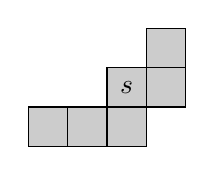
\begin{tikzpicture}
        \shadesquare{1}{1};
        \shadesquare{2}{1};
        \shadesquare{3}{1};
        \shadesquare{3}{2};
        \shadesquare{4}{2};
        \shadesquare{4}{3};
        \places{3}{2}
        \end{tikzpicture}
    \caption{An example of a non-decomposable board.}
    \label{nondecomposable}
\end{figure}

\textsc{Case 1:} If there is a rook on $s$, define $B_{s}^*$ to be the subboard of $B$ given by removing $s$ as well as all squares in the same row and column as $s$. Then there remain $k-1$ rooks to placed on $B_{s}^*$.  We define the two disjoint subboards as we see in our example below as $B_{s_1}^*$ and $B_{s_2}^*$.

\pagebreak
\begin{figure}[!h]
    \centering
    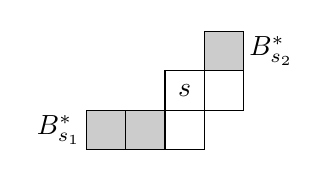
\begin{tikzpicture}
        \shadesquare{1}{1};
        \shadesquare{2}{1};
        \unshadesquare{3}{1};
        \unshadesquare{3}{2};
        \unshadesquare{4}{2};
        \shadesquare{4}{3};
        \places{3}{2}
        \placelabel{-0.2}{1}{$B_{s_1}^*$}
        \placelabel{5.2}{3}{$B_{s_2}^*$}
    \end{tikzpicture}
    \caption{The subboards created from the board in Figure \ref{nondecomposable} by placing a rook on $s$.}
    \label{case1}
\end{figure}

\textsc{Case 2:} If there is not a rook on $s$, define $B_s$ as the subboard of $B$ created when the square $s$ is removed from $B$. Then there remain $k$ rooks to be placed on $B_s$. We can define the two disjoint subboards as created in this example case as $B_{s_1}$ and $B_{s_2}$.

\begin{figure}[!h]
    \centering
    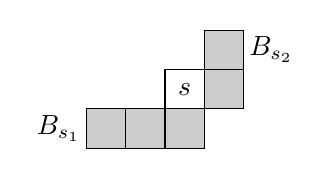
\begin{tikzpicture}
        \shadesquare{1}{1};
        \shadesquare{2}{1};
        \shadesquare{3}{1};
        \unshadesquare{3}{2};
        \shadesquare{4}{2};
        \shadesquare{4}{3};
        \places{3}{2}
        \placelabel{-0.2}{1}{$B_{s_1}$}
        \placelabel{5.2}{3}{$B_{s_2}$}
    \end{tikzpicture}
    \caption{The subboards created from the board in Figure \ref{nondecomposable} by removing $s$ (such that no rook can be placed on $s$).}
    \label{case2}
\end{figure}

Since these two cases represent whether or not there is a rook on $s$, they are mutually exclusive. So we can take the total number of ways to place $k$ rooks on $B$ as the sum of the number of ways to do so given that one of these rooks is not placed on $s$ and the number of ways to do so given that one of these rooks is placed on $s$. 
\begin{lemma} \label{recurrence}
    The rook polynomial of a board $B$ with a square marked $s$ as described above is given by
    \begin{equation} \label{ndcp}
        r_k(B) = r_k(B_s) + r_{k-1}(B_{s}^*)
    \end{equation}
\end{lemma}


Note that observing the the recurrence relation for $k = 0$ requires defining the $r_{-1}(B)$ term for $r_{k-1}(B_{s}^*)$, which is undefined. So the recurrence only holds for $k \geq 1$.

We can use Lemma 2 to calculate the number of ways to put two rooks on our example board:
\begin{align*}
    r_2(B) &= r_2(B_s) + r_{2-1}(B_{s}^*) \\
    & = r_2(B_{s_1})r_0(B_{s_2}) + r_1(B_{s_1})r_1(B_{s_2}) + r_0(B_{s_1})r_2(B_{s_2}) \\ &+ r_1(B_{s_1}^*)r_0(B_{s_2}^*) + r_0(B_{s_1}^*)r_1(B_{s_2}^*) \\
    & = ((0)(1) + (3)(2) + (1)(0)) + ((2)(1) + (1)(1)) \\
    & = 6 + 3 \\
    & = 9
\end{align*}

\pagebreak
\begin{theorem} The rook polynomial for a non-decomposable board with a given square labeled $s$ is equal to the sum of the rook polynomial of the board $B_s$ where $s$ is removed and the rook polynomial of the board $B_s^*$ where $s$ and every square in the same row or column as $s$ are removed (as if a rook has been placed at $s$) multiplied by $x$.
    \begin{equation} \label{thm2}
        R(x, B) = R(x, B_s) + x R(x, B_{s}^*)
    \end{equation}
\end{theorem}
\textsc{Note:} It is useful to choose an $s$ which breaks up the board as evenly as possible into two subboards. Then, the problem of finding $r_k(B)$ can be split into two cases as detailed above.

\begin{proof}
    Recall, we have from the definition of a rook polynomial that $R(x,B) = \sum_{k=0}^{\infty} r_k(B) x^k$. Thus,
    
    \begin{align*}
        R(x,B) &= \sum_{k=0}^{\infty} r_k(B) x^k \\
        &= 1 + \sum_{k=1}^{\infty} r_k(B) x^k \\
        &= 1 + \sum_{k=1}^{\infty} \left[ r_k(B_s) + r_{k-1}(B_{s}^*) \right] x^k \\ 
        &= 1 + \sum_{k=1}^{\infty} r_k(B_s) x^k + \underbrace{\sum_{k=1}^{\infty} r_{k-1}(B_{s}^*) x^k}_{\text{Let $k=k+1$}} \\
        &= 1 +\sum_{k=1}^{\infty} r_k(B_s) x^k + \sum_{k+1=1}^{\infty} r_{(k+1)-1}(B_{s}^*) x^{k+1} \\
        &= 1 + \sum_{k=1}^{\infty} r_k(B_s) x^k + x\sum_{k=0}^{\infty} r_{k}(B_{s}^*) x^{k} \\
        &= 1 + \sum_{k=1}^{\infty} r_k(B_s) x^k + xr_{0}(B_s^*) x^{0} + x\sum_{k=1}^{\infty} r_{k}(B_{s}^*) x^{k} \\
        &= 1 + \sum_{k=1}^{\infty} r_k(B_s) x^k + x + x\sum_{k=1}^{\infty} r_{k}(B_{s}^*) x^{k} \\
        &= 1 + \sum_{k=1}^{\infty} r_k(B_s) x^k + x \left[1 + \sum_{k=1}^{\infty} r_{k}(B_{s}^*) x^{k} \right] \\
        &= \sum_{k=0}^{\infty} r_k(B_s) x^k + x \left[ \sum_{k=0}^{\infty} r_{k}(B_{s}^*) x^{k} \right] \\
        &= R(x,B_s) + xR(x,B_s^*)
    \end{align*}
    
    
\end{proof}

\section{Application of Theorems 1 and 2 to a complex board.} \label{application}

We now have the tools to calculate the rook polynomials of more complicated boards. Figure \ref{scattered} shows such a board, which will be denoted $B$.

\begin{figure}[!h]
    \centering
    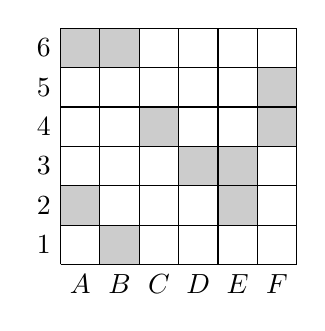
\begin{tikzpicture}
    \drawgrid{6}{6}
    
    \shadesquare{1}{2}
    \shadesquare{1}{6}
    \shadesquare{2}{1}
    \shadesquare{2}{6}
    \shadesquare{3}{4}
    \shadesquare{4}{3}
    \shadesquare{5}{2}
    \shadesquare{5}{3}
    \shadesquare{6}{4}
    \shadesquare{6}{5}
    
    \foreach \i in {1, 2, 3, 4, 5, 6} \labelrow{\i}{\i};
    \labelcol{1}{$A$}
    \labelcol{2}{$B$}
    \labelcol{3}{$C$}
    \labelcol{4}{$D$}
    \labelcol{5}{$E$}
    \labelcol{6}{$F$}
    \end{tikzpicture}
    \caption{A relatively complex board $B$.}
    \label{scattered}
\end{figure}

Before we can begin to divide this board into disjoint subboards, we ought to simplify the work ahead by clustering available squares as much as possible. A good deal of copying and checking of work may result in a clustered board similar to that in Figure \ref{organized}.

\begin{figure}[!h]
    \centering
    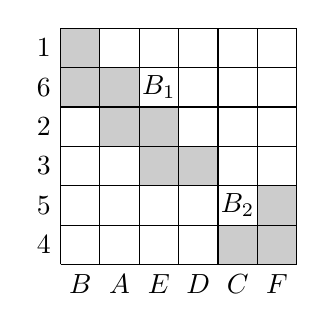
\begin{tikzpicture}
    \drawgrid{6}{6}
    \shadesquare{1}{6}
    \shadesquare{1}{5}
    \shadesquare{2}{5}
    \shadesquare{2}{4}
    \shadesquare{3}{4}
    \shadesquare{3}{3}
    \shadesquare{4}{3}
    \shadesquare{5}{1}
    \shadesquare{6}{2}
    \shadesquare{6}{1}
    
    \labelrow{1}{4}
    \labelrow{2}{5}
    \labelrow{3}{3}
    \labelrow{4}{2}
    \labelrow{5}{6}
    \labelrow{6}{1}
    \labelcol{1}{$B$}
    \labelcol{2}{$A$}
    \labelcol{3}{$E$}
    \labelcol{4}{$D$}
    \labelcol{5}{$C$}
    \labelcol{6}{$F$}
    
    \placelabel{3}{5}{$B_1$}
    \placelabel{5}{2}{$B_2$}
    
    \end{tikzpicture}
    \caption{The board $B$ from Figure \ref{scattered} rearranged to illustrate clustering and divided into disjoint subboards $B_1$ and $B_2$.}
    \label{organized}
\end{figure}

Now, we can see in Figure \ref{organized} that the board can be broken up into two disjoint subboards $B_1$ and $B_2$, as labeled in the figure. Thus, by Theorem 1, we have that $$R(x,B) = R(x,B_1)R(x,B_2)$$
The problem is now to calculate the rook polynomials of $B_1$ and $B_2$.

\begin{figure}[!h]
    \centering
    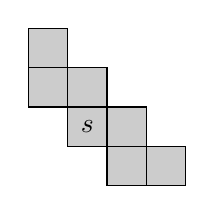
\begin{tikzpicture}
    \shadesquare{1}{4}
    \shadesquare{1}{3}
    \shadesquare{2}{3}
    \shadesquare{2}{2}
    \shadesquare{3}{2}
    \shadesquare{3}{1}
    \shadesquare{4}{1}
    \places{2}{2}
    \end{tikzpicture}
    \caption{The subboard $B_1$ with $s$ marked.}
    \label{B1}
\end{figure}

Beginning with $B_1$, we would like a way to split the subboard into two disjoint subboards. Theorem 2 gives us a way to do so by marking the square at coordinates $(A,2)$ as $s$, as shown in Figure \ref{B1}, so that $$R(x,B_1) = R(x,B_s) + xR(x,B_s^*)$$

By Theorem 2, we consider these two cases:

\textsc{Case 1:} A rook is placed on the square marked $s$. In this case, we now have two disjoint subboards $B_{s_1}^*$ and $B_{s_2}^*$, as shown in Figure \ref{Bs*}.

\begin{figure}[!h]
    \centering
    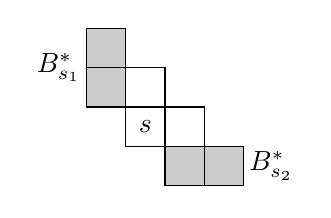
\begin{tikzpicture}
    \shadesquare{1}{4}
    \shadesquare{1}{3}
    \unshadesquare{2}{3}
    \unshadesquare{2}{2}
    \unshadesquare{3}{2}
    \shadesquare{3}{1}
    \shadesquare{4}{1}
    \places{2}{2}
    \placelabel{-.2}{3.5}{$B_{s_1}^*$}
    \placelabel{5.2}{1}{$B_{s_2}^*$}
    \end{tikzpicture}
    \caption{The subboard $B_{s}^*$, which is a subboard of $B_1$ where we assume a rook is placed at the square marked $s$. We may now divide $B_{s}^*$ into two subboards $B_{s_1}^*$ and $B_{s_2}^*$.}
    \label{Bs*}
\end{figure}

We can use the same procedure as we did to calculate the rook polynomial of Figure \ref{2by2} to find the rook polynomials of $B_{s_1}$ and $B_{s_2}$. Since these are disjoint subboards, we also have from Theorem 1 that $R(x,B_s^*) = R(x,B_{s_1}^*)R(x,B_{s_2}^*)$.
\begin{align*}
R(x, B_{s}^*) &= R(x, B_{s_1}^*)R(x, B_{s_2}^*) \\
R(x, &B_{s_1}^*) = r_0(B_{s_1}^*) + x(r_1(B_{s_1}^*))= (1 + 2x) \\
R(x, &B_{s_2}^*) = r_0(B_{s_2}^*) + x(r_1(B_{s_2}^*))= (1 + 2x) \\
R(x, B_{s}^*) &= (1 + 2x)(1 + 2x) \\
&= 1 + 4x + 4x^2
\end{align*}

\textsc{Case 2:} No rook is placed on the square marked $s$. In this case, we have two disjoint subboards $B_{s_1}$ and $B_{s_2}$, as shown in Figure \ref{Bs}.

\begin{figure}[!h]
    \centering
    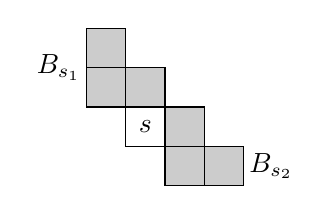
\begin{tikzpicture}
    \shadesquare{1}{4}
    \shadesquare{1}{3}
    \shadesquare{2}{3}
    \unshadesquare{2}{2}
    \shadesquare{3}{2}
    \shadesquare{3}{1}
    \shadesquare{4}{1}
    \places{2}{2}
    \placelabel{-.2}{3.5}{$B_{s_1}$}
    \placelabel{5.2}{1}{$B_{s_2}$}
    \end{tikzpicture}
    \caption{The subboard $B_s$, a subboard of $B_1$. We assume no rook will be placed on $s$ and accordingly divide $B_s$ into two subboards $B_{s_1}$ and $B_{s_2}$.}
    \label{Bs}
\end{figure}
The rook polynomials of $B_{s_1}$ and $B_{s_2}$ can be calculated relatively easily. We can again apply Theorem 1 because $B_{s_1}$ and $B_{s_2}$ are disjoint.

\begin{align*}
R(x,B_s) &= R(x,B_{s_1})R(x,B_{s_2}) \\
R(x, &B_{s_1}) = r_0(B_{s_1}) + x(r_1(B_{s_1})) + x^2(r_2(B_{s_1})) = 1 + 3x + x^2 \\
R(x, &B_{s_2}) = r_0(B_{s_2}) + x(r_1(B_{s_2})) + x^2(r_2(B_{s_2})) 1 + 3x + x^2 \\
R(x, B_s) &= (1 + 3x + x^2)(1 + 3x + x^2) \\
&= 1 + 6x + 11x^2 + 6x^3 + x^4
\end{align*}
Thus, we may now use Theorem 2 to calculate the rook polynomial for $B_1$.
\begin{align*}
    R(x,B_1) &= R(x, B_s) + x(R(x, B_{s}^*)) \\
    &= (1 + 6x + 11x^2 + 6x^3 + x^4) + x(1 + 4x + 4x^2) \\
    &= 1 + 7x + 15x^2 + 10x^3 + x^4
\end{align*}

\begin{figure}[!h]
    \centering
    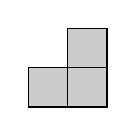
\begin{tikzpicture}
    \shadesquare{1}{1}
    \shadesquare{2}{2}
    \shadesquare{2}{1}
    \end{tikzpicture}
    \caption{The subboard $B_2$}
    \label{B2}
\end{figure}

We can easily determine the rook polynomial for the subboard $B_2$. That is: 
\begin{align*}
R(x, B_2) &= r_0(B_2) + r_1(B_2)x + r_2(B_2)x^2 + ... \\
&= 1 + 3x + x^2 + 0... \\
&= 1 + 3x + x^2
\end{align*}

Now that we have $R(x, B_1)$ and $R(x, B_2)$, we can finally apply Theorem 1 to find $R(x, B)$ for our original board $B$.
\begin{align*}
    R(x, B) &= R(x, B_1)R(x, B_2) \\
    R(x, B) &= (1 + 7x + 15x^2 + 10x^3 + x^4)(1 + 3x + x^2) \\
    R(x, B) &= 1 + 10x + 37x^2 + 62x^3 + 46x^4 + 13x^5 + x^6
\end{align*}

\section{References} \label{references}

Tucker, Alan. Applied Combinatorics (John Wiley \& Sons, Inc.), pages 329-339. 

\end{document}
